\chapter{Transmissão de dados HDMI}\label{chap:chap3}

Este capítulo descreve o trabalho realizado para cumprir a primeira parte do projeto: obter uma conexão HDMI entre recetor e transmissor. São descritas as várias configurações das placas HDMI disponíveis e ainda as arquiteturas desenvolvidas e implementadas para cumprir esta parte do projeto. 

\section{Infraestrutura do \textit{Hardware} utilizado} \label{sec:hardware}

Tal como mencionado na subsecção \ref{sec:HDMIinFPGA}, para receber os dados provenientes do cabo HDMI e fazer a sua seleção são utilizadas duas placas HDMI (TB-FMCH-HDMI2 RX e TB-FMCH-HDMI2 TX) que, através das suas entradas e saídas FMC de alta velocidade conseguem enviar e receber da FPGA os sinais de imagem e som. Nas figuras \ref{fig:rx} e \ref{fig:tx} é possível visualizar o recetor (TB-FMCH-HDMI2 RX) e o transmissor (TB-FMCH-HDMI2 TX) HDMI utilizados neste projeto. Em conjunto, estas duas placas são designadas apenas por TB-FMCH-HDMI2. Estas mesmas placas são constituídas por conectores HDMI onde é recebido o sinal HDMI que de seguida é enviado para um recetor ou transmissor, ADV7612 (cuja \textit{data sheet} está referenciada em \cite{R038}) no caso do recetor e ADV7511 (cuja \textit{data sheet} está referenciada em \cite{R039}) no caso do transmissor. Finalmente os sinais provenientes do recetor/transmissor são enviados para uma FPGA da placa (XC6SLX45-3FGG484C) que, consoante a sua configuração, envia pelos conectores FMC os sinais de áudio e vídeo.

\begin{figure}[h!]
	\begin{center}
		\leavevmode
		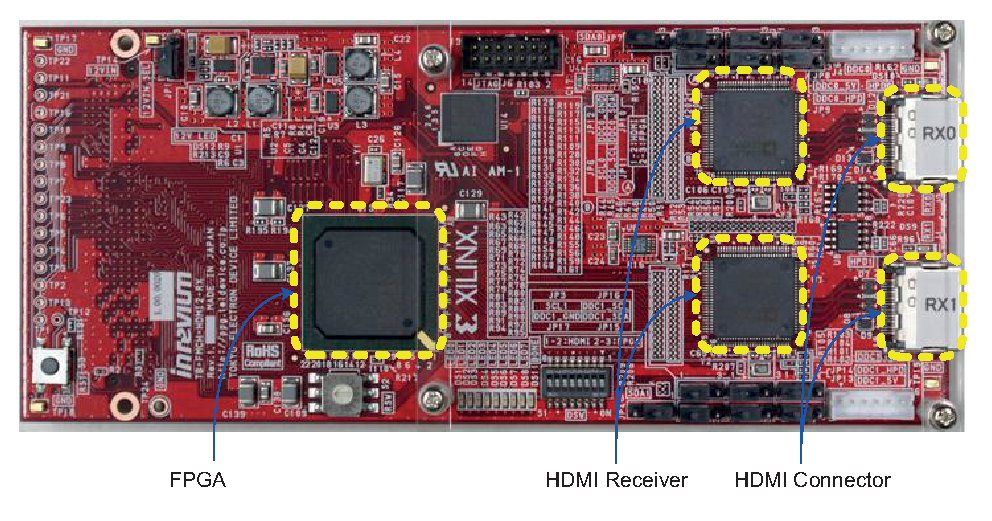
\includegraphics[width=0.75\textwidth]{placa_HDMI_rx_vet}
		\caption[Placa HDMI recetora]{Placa HDMI recetora (retirada de \cite{R009})}
		\label{fig:rx}
	\end{center}
\end{figure}

\begin{figure}[h!]
	\begin{center}
		\leavevmode
		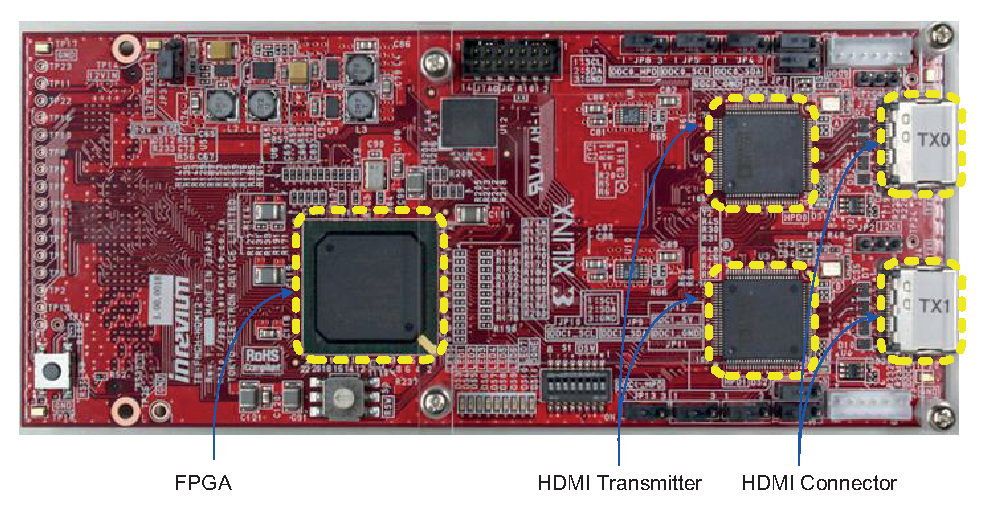
\includegraphics[width=0.75\textwidth]{placa_HDMI_tx_vet}
		\caption[Placa HDMI transmissora]{Placa HDMI transmissora (retirada de \cite{R009})}
		\label{fig:tx}
	\end{center}
\end{figure}


As placas possuem ainda uma PROM (\textit{Programmable read-only memory}) XCF16PFSG48C de configuração reprogramável que permite armazenar o \textit{bitstream}\footnote{Ficheiro de dados binários que representa toda a conectividade e encaminhamento dos recursos lógicos da FPGA para uma determinada arquitetura desenvolvida} que configura a FPGA do modo que se pretende. É esta FPGA integrada que em cada placa (RX e TX) é responsável pela seleção e envio ou receção dos dados pretendidos para/ou dos conectores FMC, e como tal é necessário que estejam configuradas para realizarem tais procedimentos. O recurso a estas memórias reconfiguráveis vem permitir uma fácil alteração da configuração da FPGA uma vez que, segundo \cite{R026}, estas memórias de leitura permitem não só armazenar os \textit{bitstreams} de configuração da FPGA, mas também podem ser reconfiguradas para outros \textit{bitstreams} de forma fácil e eficiente.

As reconfigurações destas memórias são realizadas através de um programador JTAG (\textit{Joint Test Action Group}) e ainda recorrendo a um \textit{software}. O \textit{software} utilizado neste projeto tem o nome de \textit{imPACT} e é disponibilizado pela \textit{Xilinx}. Após a conexão do conector JTAG à respectiva placa e ao computador (através de uma porta USB - \textit{Universal Serial Bus}) é necessário inicializar o \textit{software} e programar a memória com o ficheiro pretendido. Em \cite{R025} são detalhadas informações acerca do programador utilizado e ainda sobre o procedimento para se reconfigurar as memórias. As alterações do modo de funcionamento das placas HDMI neste projeto baseiam-se nesse documento.

\subsection{Configurações da FPGA} \label{subsec:HDMIconfig}

A FPGA \textit{Spartan-6} (XC6SLX45-3FGG484C) das placas tem três configurações disponíveis. Estas variam não só no suporte de imagem e som que possuem, mas podem igualmente variar no número de bits por imagem que podem ter. Nas secções seguintes serão abordadas as configurações disponíveis e como se pode tirar partido das mesmas no projeto desenvolvido.

\subsubsection{Configuração por omissão} \label{subsubsec:HDMIconfigdefault}

Esta configuração vem previamente escrita na memória PROM de fábrica e acaba por ser a mais simples de todas. Os dados enviados pelos conectores FMC são apenas referentes à imagem. As tabelas \ref{table:HDMIdataRX} e \ref{table:HDMIdataTX} identificam as portas às quais são atribuídas os sinais de dados de imagem HDMI tanto na placa recetora como na transmissora.

Esta configuração suporta a transmissão de imagens RGB (\textit{Red Green Blue}) com 10 bits. Assim sendo, tal como referido em \cite{R009}, independentemente da formatação das imagens da fonte HDMI o recetor ADV7612 integrado na placa recetora HDMI converte a imagem para o formato RGB e transmite de maneira a enviar os dados em apenas 10 bits. A tabela \ref{table:HDMIdefaultSimplified}, adaptada de \cite{R009}, apresenta brevemente quais as portas das placas utilizadas e que sinais são transmitidos nas mesmas. Todavia é possível encontrar na secção \ref{ap1:default} do anexo \ref{ap1:HDMI} mais detalhes relativamente a estes dados. Os nomes dos sinais apresentados nestas tabelas são referentes aos sinais em TB-FMCH-HDMI2 (tanto TX como RX), e como tal quando se faz referência à FPGA nestas tabelas estas correspondem às que estão integradas nas placas HDMI. 

\begin{table}[h!]
	\centering
	\caption[Descrição e localização dos pinos de TB-FMCH-HDMI2 configurada por omissão]{Descrição e localização dos pinos de TB-FMCH-HDMI2 configurada por omissão}
	\label{table:HDMIdefaultSimplified}
	\resizebox{\textwidth}{!}{%
		\begin{tabular}{@{}llll@{}}
			\toprule
			\multicolumn{1}{c}{\textbf{PINO}} & \multicolumn{1}{c}{\textbf{FPGA -\textgreater FMC (RX)}} & \multicolumn{1}{c}{\textbf{FMC -\textgreater FPGA (TX)}} & \multicolumn{1}{c}{\textbf{Descrição}} \\ \midrule
			CLK0\_M2C\_P            & RX\#0\_LLC                                     & TX\#0\_DCLK                                & Sinal de relógio dos píxeis   \\
			LA00\_P\_CC             & RX\#0\_VSYNC                                   & TX\#0\_VSYNC                               & Sincronização Vertical        \\
			LA01\_P\_CC             & RX\#0\_HSYNC                                   & TX\#0\_HSYNC                               & Sincronização Horizontal      \\
			LA02\_P                 & RX\#0\_DE                                      & TX\#0\_DE                                  & Sinal de Dados Ativos         \\
			LA03\_P a LA32\_P       & RX\#0\_P0 a RX\#0\_P29                         & TX\#0\_D0 a TX\#0\_D29                     & Pixel de Imagem               \\ \bottomrule
		\end{tabular}%
	}
\end{table}

É de notar ainda que esta configuração é capaz de suportar até dois canais (RX0 e TX0, RX1 e TX1). Contudo nesta tabela apenas são apresentados os dados correspondentes ao canal 0 pois apenas é utilizado um canal neste projeto. 

Apesar de ser uma configuração simples, uma vez que apenas são transmitidos sinais de imagem em formato RGB é uma configuração que é utilizada numa fase inicial em algumas arquiteturas implementadas que serão descritas na secção \ref{sec:HDMIarquiteturas}.

\subsubsection{Suporte de um canal de imagem e áudio} \label {subsubsec:HDMIconfig+audio}

Para além da configuração descrita em \ref{subsubsec:HDMIconfigdefault} que apenas suporta a transmissão de imagem, existe ainda uma configuração capaz de suportar não só a transmissão de imagem mas também de som. A configuração que é escrita na PROM da placa recetora para programar a FPGA controla o recetor ADV7612 de maneira a conseguir transmitir imagens no formato YCbCr\footnote{É um espaço de cores usado em imagens digitais. \textit{Y} representa o brilho da imagem, \textit{Cb} e \textit{Cr} representam a diferença entre o brilho e as cores azul e vermelho respetivamente} ou RGB com 12 bits e também fazer a transmissão do áudio em formato $I^{2}$S (\textit{Inter-IC Sound}). O mesmo acontece na placa transmissora para ser capaz de receber estas configurações.

Assim como referido em \cite{R014}, neste caso a configuração da imagem está dependente da fonte HDMI e é transmitida pelas placas tal como é emitida pela fonte. No caso do som, este é sempre transmitido em formato $I^{2}$S, o que implica não só a transmissão dos dados de áudio, mas também sinais de relógio necessários à sua transmissão.

Na tabela \ref{table:HDMIaudiosuportSimplified} são brevemente apresentadas as portas e os sinais usados com este tipo de configuração. Na secção \ref{ap1:HDMIconfig+audio} no anexo \ref{ap1:HDMI} é apresentada uma tabela semelhante a esta, mas que inclui mais detalhes relativamente aos pinos usados. Ambas as tabelas foram adaptadas de \cite{R014} onde são apresentados todos os detalhes dos conectores FMC das placas.

\begin{table}[h!]
	\caption{Descrição e localização dos pinos de TB-FMCH-HDMI2 configurada para um canal de imagem e áudio}
	\label{table:HDMIaudiosuportSimplified}
	\centering
	\resizebox{\textwidth}{!}{%
		\begin{tabular}{@{}llll@{}}
			\toprule
			\multicolumn{1}{c}{\textbf{PINO}} & \multicolumn{1}{c}{\textbf{FPGA -\textgreater FMC (RX)}} & \multicolumn{1}{c}{\textbf{FMC -\textgreater FPGA (TX)}} & \multicolumn{1}{c}{\textbf{Descrição}} \\ \midrule
			CLK0\_M2C\_P                      & RX\#0\_LLC                                               & TX\#0\_DCLK                                              & Sinal de relógio dos píxeis            \\
			LA00\_P\_CC                       & RX\#0\_VSYNC                                             & TX\#0\_VSYNC                                             & Sincronização Vertical                 \\
			LA01\_P\_CC                       & RX\#0\_HSYNC                                             & TX\#0\_HSYNC                                             & Sincronização Horizontal               \\
			LA02\_P                           & RX\#0\_DE                                                & TX\#0\_DE                                                & Sinal de Dados Ativos                  \\
			LA03\_P a LA32\_P                 & RX\#0\_P0 a RX\#0\_P29                                   & TX\#0\_D0 a TX\#0\_D29                                   & Pixel de Imagem do bit 0 ao 29         \\
			LA00\_N\_CCa LA01\_N\_CC          & RX\#0\_InputVideoStatus                                  & TX\#0\_InputVideoStatus                                  & Formato de video (2D/3D)               \\
			LA19\_N                           & RX\#0\_MCLK                                              & TX\#0\_MCLK                                              & \textit{Master Clock} de som                    \\
			LA20\_N                           & RX\#0\_SCLK                                              & TX\#0\_SCLK                                              & S\textit{erial Clock} de som                    \\
			LA21\_N a LA26\_N                 & RX\#0\_AP0 a RX\#0\_AP5                                  & TX\#0\_AP0 a TX\#0\_AP5                                  & Dados de som                           \\
			LA27\_N a LA32\_N                 & RX\#0\_P30 a RX\#0\_P35                                  & TX\#0\_P30 a TX\#0\_P35                                  & Pixel de imagem do bit 30 ao 35        \\ \bottomrule
		\end{tabular}%
	}
\end{table}

Os dados referentes ao som transmitidos pela placa recetora e recebidos de seguida pela placa emissora estão também mencionados com mais detalhe na secção \ref{ap1:HDMIconfig+audio} do anexo \ref{ap1:HDMI}. Esta configuração é capaz de transmitir e receber dados no formato $I^{2}$S cujas especificações se encontram em \cite{R027}, onde são definidos os sinais transmitidos aquando da utilização deste formato:

\begin{enumerate}
	\item \textbf{\textit{Continuous Serial Clock} (SCK):} Este sinal é por vezes reconhecido pelo nome de \textit{Bit Clock} e é um sinal de relógio referente aos dados de som em série transmitidos pelos canais AP1, AP2, AP3 e AP4.
	
	\item \textbf{\textit{Word Select} (WS)}: Este sinal é por vezes também conhecido por \textit{Left/Right Clock} e é um sinal que indica o canal de som (esquerdo ou direito) que está a ser transmitido através dos dados em série recebidos ou enviados nas portas AP1, AP2, AP3 e AP4. É denominado sinal de relógio porque geralmente alterna entre 0 e 1 periodicamente. Porém, isto pode não acontecer, tal como referido em \cite{R027}. 
	
	\item \textbf{\textit{Serial Data}}: Sinais que transportam os dados de áudio.

\end{enumerate}

Na figura \ref{fig:i2s_audio} são ilustrados os sinais referentes ao áudio descritos previamente. O sinal \textit{SCLK} (\textit{Serial Clock}) é referente ao sinal "\textit{Continuous Serial Clock}", o sinal \textit{LRCLK} (\textit{Left/Right Clock}) refere-se ao sinal "\textit{Word Select}" e ainda \textit{ISx }refere-se ao sinal "\textit{Serial Data}". É de notar que os dados de som alternam à frequência do sinal \textit{SCLK} que possui uma frequência 64 vezes superior à de \textit{LRCLK}. Segundo \cite{R014} a frequência deste é de \SI{48}{\kilo\hertz} e por isso o sinal \textit{SCLK} possui uma frequência de aproximadamente de  \SI{3.072}{\mega\hertz}.

\begin{figure}[h!]
	\begin{center}
		\leavevmode
		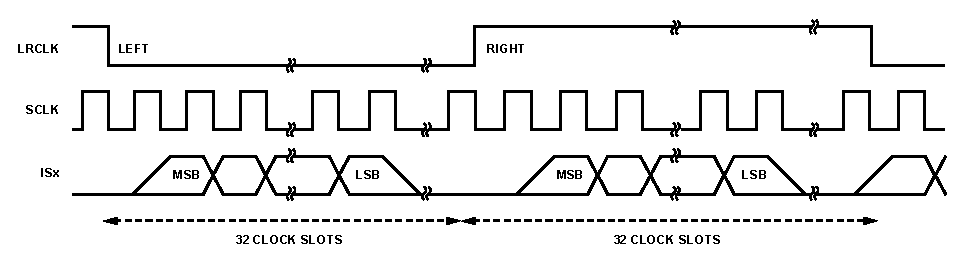
\includegraphics[width=1.0\textwidth]{audio_i2s}
		\caption[IRepresentação dos sinais de som transmitidos no formato $I^{2}$S]{Representação dos sinais de som transmitidos no formato $I^{2}$S (retirada de \cite{R016})}
		\label{fig:i2s_audio}
	\end{center}
\end{figure}

Na placa recetora HDMI que envia os dados para a FPGA Virtex-7, é também enviado o sinal \textit{Master Clock} que corresponde a um sinal de relógio de referência dos sinais de áudio da entrada e ainda os dados de áudio em AP0. É mencionado em \cite{R016} que estes dois sinais são referentes ao som no formato SPDIF (\textit{Sony/Philips Digital Interface Format}) e por isso não serão abordados neste projeto uma vez que as placas apenas suportam o formato $I^{2}$S.

Para além de dados de som e imagem são transmitidos dois bits com informação relativa ao estado do vídeo transmitido. Estes dados indicam o tipo e formato de vídeo que está a ser transmitido e devem de seguida ser recebidos na placa transmissora. As combinações dos dois bits definem o estado do vídeo e são detalhadas em \cite{R014}.

Esta configuração é bastante útil e será utilizada em diversas arquiteturas desenvolvidas uma vez que possui duas grandes vantagens: é capaz de suportar som e ao mesmo tempo não limita o formato da imagem transmitida a RGB. Em contrapartida, apenas suporta um canal (ao contrário da anterior), mas tal não é um problema pois apenas se pretende obter a transmissão num único canal entre dispositivo de fonte e dispositivo final HDMI. 


\subsubsection{Suporte de dois canais de imagem melhorado} \label{subsubsec:HDMIconfigMelhorado}


Esta configuração é capaz de suportar a transmissão de imagens em dois canais, tal como a configuração apresentada em \ref{subsubsec:HDMIconfigdefault}, mas com algumas melhorias. A principal diferença consiste na capacidade de transmitir não só imagens em formato RGB mas também em YCbCr num dos canais. Na secção \ref{ap1:HDMIconfigMelhorado} do anexo \ref{ap1:HDMI} são apresentados detalhes relativamente a todos os sinais transmitidos pelas placas com esta configuração.

Esta configuração na placa recetora transmite no canal 0 (RX0) imagens tanto no formato RGB como YCbCr de 10 bits por cor e respetivos sinais de controlo. Relativamente ao canal 1 dessa mesma placa (RX1) apenas é possível transmitir imagens em formato RGB de 10 bits por cor e os seus sinais de controlo. Para além disso, para cada canal são transmitidos dois bits que identificam o estado do vídeo que é transmitido, tal como já acontecia na configuração descrita em \ref{subsubsec:HDMIconfig+audio}. Quanto à placa transmissora quando configurada desta forma é capaz de receber nos dois canais (TX0 e TX1) imagens no formato RGB ou YCbCr com 10 bits por cor. 

Esta configuração traz vantagens relativamente à primeira apresentada em \ref{subsubsec:HDMIconfigdefault}, uma vez que é capaz de suportar imagens no formato YCbCr, contudo não suporta som, e portanto não é utilizada em nenhuma arquitetura desenvolvida neste projeto. 

%Na tabela \ref{table:HDMI1canal_melhorado} o canal 1 não é apresentado pois não é relevante para o projeto (visto que só se faz uso de um canal).
% Apesar de na tabela \ref{table:HDMI1canal_melhorado} o canal 1 definir os seus bits apenas para o caso de RGB, este canal também suporta na placa transmissora o formato YCbCr (e por isso a atribuição dos bits para TX1 assemelham-se ao canal TX0). Tal não é suportado no canal 1 da placa HDMI recetora (RX1) e por esse motivo a tabela está assim apresentada. À semelhança da placa recetora, a placa transmissora recebe 2 bits relativos à informação do vídeo que está a ser transferido, tal como a tabela \ref{table:HDMI1canal_melhorado} sugere.

\subsection{Configuração dos interruptores}

Nesta subsecção são descritas as funcionalidades dos interruptores presentes nas placas HDMI. Estes precisam de estar definidos com determinadas combinações tanto no recetor como no transmissor para que possam enviar e receber as imagens nos formatos que o utilizador pretende.
%Tal é necessário definir para que os recetores e transmissores presentes nas placas possam enviar e receber imagens nos formatos que o utilizador pretende. 

Existem 8 interruptores que podem ser definidos pelo utilizador. Os interruptores entre S1-1 e S1-4 têm como função selecionar o tipo de formato que sai do recetor ADV7612 ou do transmissor ADV7511 integrado na respetiva placa. Relativamente aos outros interruptores, raramente são utilizados e quando o são, a sua função não é relevante para o projeto, por isso não são especificadas neste documento. As diversas combinações estão apresentadas no anexo \ref{ap4:switches}.


\section{Arquiteturas Desenvolvidas} \label{sec:HDMIarquiteturas}

Nesta secção são descritas as arquiteturas desenvolvidas e implementadas na FPGA referentes à comunicação direta entre as placas HDMI. Todas as configurações que foram apresentadas na secção \ref{sec:hardware} deste capítulo são agora exploradas. Para cada arquitetura desenvolvida é apresentada a sua conceção, desenvolvimento e também os resultados obtidos. No final é feita uma comparação de resultados relativamente aos recursos utilizados por cada uma das arquiteturas na FPGA.


\subsection{Transmissão de uma imagem gerada na FPGA} \label{subsub:planA}

Numa fase inicial do projeto optou-se por simplificar a transmissão e utilizou-se apenas a placa transmissora HDMI configurada por omissão. Construiu-se em Verilog um bloco capaz de gerar uma imagem para ser transmitida, mais especificamente uma barra de cores, e utilizou-se essa imagem para ser transmitida pelos conectores FMC.

\subsubsection*{Conceção e Desenvolvimento}

O bloco gerador de uma barra de cores foi adaptado de uma arquitetura disponibilizada pela \textit{Inrenvium} aquando da compra das placas. Apesar de ter sido ligeiramente adaptado para este caso em específico, este baseia-se essencialmente numa máquina de estados que vai contando as linhas e as colunas para que possa enviar não só os valores das cores de cada píxel, mas também os sinais de controlo como a sincronização vertical (\textit{vsync}), a sincronização horizontal(\textit{hsync}) e ainda o valor de píxeis ativos (\textit{enable}).

Para que se entenda mais facilmente como e quando se transmitem os sinais de controlo da imagem e também o valor dos píxeis é demonstrado na figura \ref{fig:colorBar_exemple} um exemplo de transmissão de uma imagem gerada na FPGA. Antes de se passar para descrição da geração da imagem, passam a ser descritos as siglas e acrónimos apresentados na figura:

\begin{enumerate}
	\item \textbf{HRES:} \textit{Horizontal Resolution} é o parâmetro que define a resolução horizontal da imagem que vai ser gerada pelo bloco, ou seja, o número de píxeis da imagem.
	
	\item \textbf{HSW:} \textit{Horizontal Sync Width} é o parâmetro que define o número de ciclos de relógio quando o sinal de sincronização horizontal  está ativo.
	
	\item \textbf{HBP:} \textit{Horizontal Back Porch} é o parâmetro que define o número de píxeis que não contêm informação útil (relativamente à cor dos mesmos) antes de começar a ser transmitida a linha de imagem.
	
	\item \textbf{HFP:} \textit{Horizontal Front Porch} é o parâmetro que define o número de píxeis que não contêm informação útil depois de ser transmitida uma linha da imagem.
	
	\item \textbf{VRES:} \textit{Vertical Resolution} é o parâmetro que define a resolução vertical da imagem que vai ser gerada pelo bloco, por outras palavras, é o número de linhas da imagem gerada.
	
	\item \textbf{VSW:} \textit{Vertical Sync Width} é o parâmetro que define o número de linhas horizontais quando o sinal de sincronização vertical está ativo.
	
	\item \textbf{VBP:} \textit{Vertical Back Porch} é o parâmetro que define o número de linhas horizontais que não contém informação útil relativamente aos píxeis antes de começarem a ser transmitidas as linhas de píxeis.
	
	\item \textbf{VFP:} \textit{Vertical Front Porch} é o parâmetro que define o número de linhas horizontais que não contém informação útil relativamente aos píxeis depois de terem sido transmitidas todas as linhas horizontais da imagem.
\end{enumerate}
	
\begin{figure}[h!]
	\begin{center}
		\leavevmode
		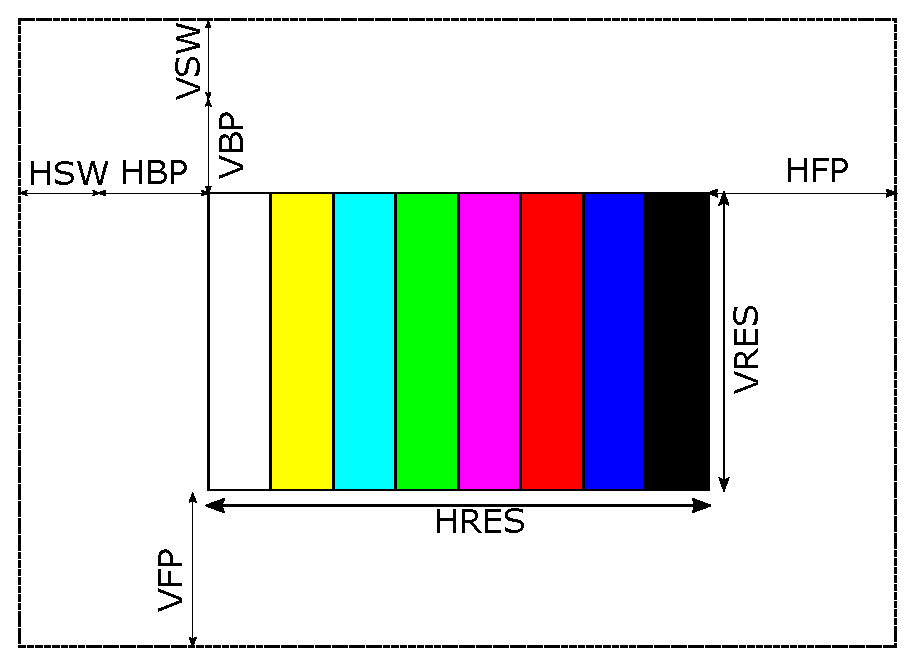
\includegraphics[width=0.90\textwidth]{exemplo_colorBar}
		\caption{Exemplo de imagem gerada pelo módulo desenvolvido}
		\label{fig:colorBar_exemple}
	\end{center}
\end{figure}

Para gerar uma imagem em \textit{FULL HD}, cuja resolução é 1920x1080 píxeis, o sinal de relógio deve ter uma frequência de \SI{148.5}{\mega\hertz} e por isso foram utilizados os seguintes valores para os parâmetros previamente descritos: HRES = 1920, HSW = 148, HBP = 44, HFP = 88,  VRES = 1080, VSW = 5, VBP = 36 e VFP = 4. Com estes valores é possível obter uma taxa de atualização vertical de 60 Hz (60 imagens por segundo).

\begin{figure}[h!]
	\begin{center}
		\leavevmode
		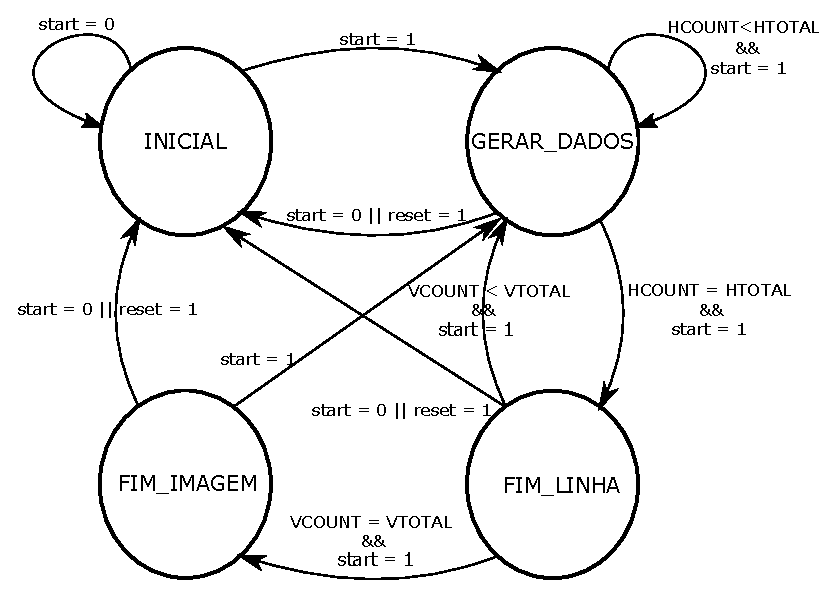
\includegraphics[width=0.8\textwidth]{colorBar_FSM}
		\caption{Máquina de estados para gerar uma barra de cores}
		\label{fig:colorBar_fsm}
	\end{center}
\end{figure}

A figura \ref{fig:colorBar_fsm} ilustra a máquina de estados desenvolvida para implementar a geração de uma barra a cores na FPGA. Os registos VCOUNT e HCOUNT de decisão na máquina de estados correspondem a contadores que vão contanto píxel a píxel até ao fim de uma linha (no caso do HCOUNT) ou então de uma imagem inteira (no caso do VCOUNT). Os valores de HTOTAL e VTOTAL não são mais do que a soma de todo o tamanho dos dados na horizontal e na vertical respetivamente. Assim sendo, para este caso em específico obtém-se os seguintes valores:
\begin{itemize}
	\item HTOTAL = HSW + HBP + HRES + HFP = 44 + 148 + 1920 + 88 = 2200
	\item VTOTAL = VSW + VBP + VRES + VFP = 5 + 36 + 1080 + 4 = 1125
\end{itemize}


Para além destes sinais de decisão para mudança de estado existem mais dois sinais no diagrama da máquina de estados presente na figura \ref{fig:colorBar_fsm} que ainda não foram mencionados que são o \textit{reset} e o \textit{start}. Estes dois sinais são botões do utilizador que lhe permite definir quando pretende que a transmissão esteja ativa ou não (através do botão \textit{start}), ou então quando pretende restabelecer os dados originais da máquina de estados (através do botão \textit{reset}). 

Existem 4 estados nesta máquina que consistem essencialmente em deteção do final de uma linha, deteção do final de uma imagem e geração de dados. Esses estados são:

\begin{enumerate}
	\item \textbf{Estado inicial:} Neste estado são configurados os parâmetros para o início de uma transmissão, ou seja, os valores de HCOUNT e VCOUNT são igualados ao valor total do tamanho horizontal e vertical respetivamente. É possível retornar a este estado estando em qualquer um dos outros desde que seja pressionado o botão  de \textit{reset}, ou então que a transmissão seja desligada pelo utilizador (\textit{start} = 0).
	
	\item \textbf{Estado para gerar dados:} Neste estado, ao flanco positivo do sinal de relógio do sistema é incrementado o valor de HCOUNT e ao mesmo tempo são gerados os dados a serem transmitidos em cada ciclo de sinal de relógio (consoante o valor de HCOUNT e VCOUNT) . Quando o valor de HCOUNT se igualar ao valor de HTOTAL, então significa que foi transmitida uma linha inteira da imagem e por isso a máquina transita de estado e o valor de HCOUNT volta a ser igualado a 1.
	
	\item \textbf{Estado de fim de linha:} Quando este estado está ativo, então uma linha da imagem foi transmitida, sendo necessário incrementar o valor de linhas totais transmitidas (incrementando 1 valor em VCOUNT) e ainda verificar se a transmissão de uma imagem completa está realizada. Caso o valor de VCOUNT se iguale ao valor de VTOTAL, então transita-se para o estado de fim de imagem e coloca-se o valor de VCOUNT a 1. Caso contrário a máquina transita para o estado que estava anteriormente.
	
	\item \textbf{Estado de fim de imagem} Quando este estado está ativo então significa que ambos os valores de HCOUNT e VCOUNT estão igualados a 1 e que por isso já foi transmitida uma imagem completa. Como tal, passa-se a transmitir uma próxima imagem transitando novamente para o estado para gerar dados.
	
\end{enumerate}

Quando a máquina de estados se encontra no estado para gerar dados, então estes são gerados nas seguintes condições:
\begin{itemize}
	\item \textbf{Sinal de sincronização vertical:} O sinal de sincronização vertical é um sinal que indica o início de transmissão de uma nova imagem e por isso é ativado pela máquina de estados quando o valor em VCOUNT se igualar ao valor de VTOTAL e quando o valor de HCOUNT se igualar ao valor de HTOTAL (final de uma imagem). Este sinal é desligado quando o valor de VCOUNT se igualar a VSW e o valor de HCOUNT se igual ao valor de HTOTAL (indica que o número de linhas em que o sinal de sincronização vertical deve estar ativo já terminou).
	
	\item \textbf{Sinal de sincronização horizontal:} O sinal de sincronização horizontal indica o início de uma nova linha e por isso deve ser ativo sempre que o valor de HCOUNT se igualar ao valor de HTOTAL (fim da emissão de uma linha). Da mesma maneira, este sinal deve ser desligado sempre que o valor de HCOUNT se igualar ao valor de HSW (indica que o período de tempo que este sinal deve estar ativo terminou).
	
	\item \textbf{Sinal de dados ativos:} Este sinal deve estar ativo sempre que se estiver a transmitir píxeis válidos, ou seja, quando estas condições se verificam:
	\begin{enumerate}
		\item O valor de VCCOUNT é maior do que a soma entre VSW e VBP.
		\item O valor de VCOUNT é menor do que a soma entre VSW, VBP, VRES e um.
		\item O valor de HCOUNT é maior do que a soma entre HSW, HBP subtraída de um valor.
		\item O valor de HCOUNT é menor do que a soma HSW, HBP e HRES.
	\end{enumerate}

	As condições 1 e 2 garantem que VCOUNT está na zona vertical que corresponde à transmissão de imagem na figura \ref{fig:colorBar_exemple}, enquanto que as condições 3 e 4 garantem o mesmo mas na zona horizontal.
	
	\item \textbf{Valor dos píxeis:} Estes sinais correspondem a um barramento de 30 bits de uma imagem RGB com 10 bits por componente de cor. Como tal, estes valores devem corresponder a cores sempre que o sinal de dados ativos estiver ativo e devem ser igualados a zero sempre que o mesmo estiver inativo.
 
\end{itemize}

\subsubsection*{Localizações das portas de saída do módulo de topo} 

\begin{figure}[h!]
	\begin{center}
		\leavevmode
		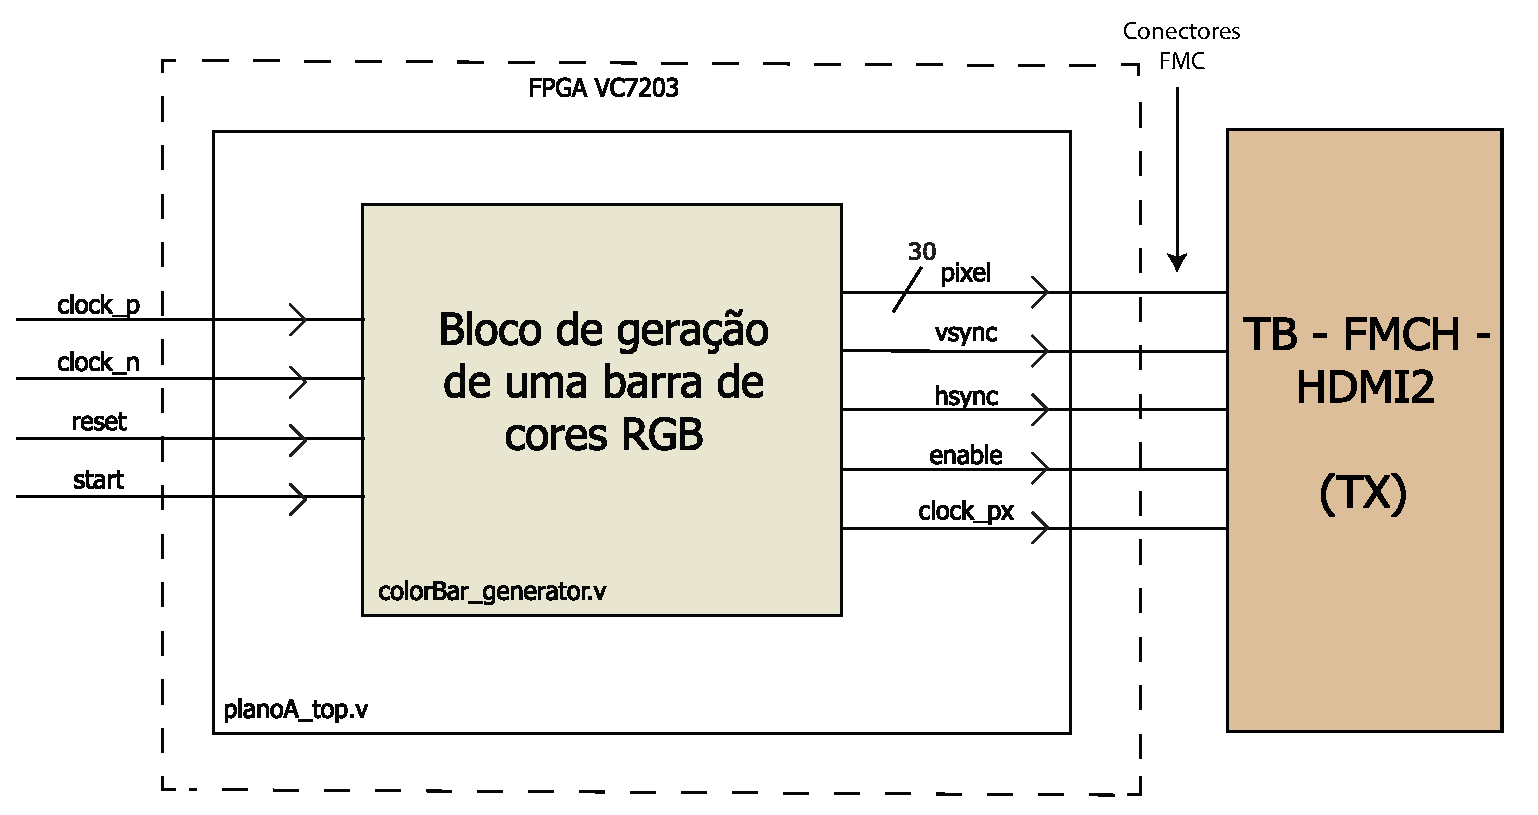
\includegraphics[width=1.0\textwidth]{planA}
		\caption{Diagrama de blocos de arquitetura que transmite uma barra de cores para a placa HDMI TX}
		\label{fig:planA}
	\end{center}
\end{figure}

Na figura \ref{fig:planA} é apresentado um diagrama de blocos da arquitetura implementada recorrendo a um módulo gerador de uma barra de cores. Este foi implementado recorrendo-se à maquina de estados apresentada anteriormente.

Nas entradas do bloco estão ligados 4 sinais sendo que dois deles correspondem a um sinal de relógio diferencial de \SI{200}{\mega\hertz} (\textit{clock\_p} corresponde ao sinal positivo e \textit{clock\_n} ao sinal negativo). Os outros dois sinais, \textit{start} e \textit{reset}, são sinais relevantes para a máquina de estados do bloco de geração de barras de cores definidos pelo utilizador e, por isso, são atribuídos a botões da FPGA. O sinal de relógio diferencial ligado às entradas deste bloco é proveniente do oscilador presente na FPGA e alimenta um módulo que coloca na sua saída um sinal de relógio de \SI{148.5}{\mega\hertz}. Esse módulo foi criado através do IP(\textit{Intellectual Property}) disponibilizado no \textit{software} VIVADO com o nome de \textit{Clocking Wizard} que vem facilitar a geração de um sinal de relógio com a frequência pretendida tendo como uma base um sinal diferencial de \SI{200}{\mega\hertz}. O sinal gerado, de \SI{148.5}{\mega\hertz}, é o principal sinal de relógio do sistema que permite a geração da barra de cores. Esta é a cadência a que os sinais são enviados para a placa HDMI transmissora.

Relativamente às saídas do módulo é possível ver na figura \ref{fig:planA} que estas se encontram diretamente ligadas à placa transmissora HDMI através dos conectores FMC. Estes sinais constituem um barramento de 30 bits que corresponde ao valor do píxel (\textit{pixel}), o sinal de sincronização horizontal (\textit{hsync}), o sinal de sincronização vertical (\textit{vsync}) e ainda o sinal de dados ativos (\textit{enable}).

Para além do desenvolvimento do código em Verilog é necessário que as portas do módulo de topo estejam atribuídas a portas físicas da FPGA. Consequentemente, é necessário definir as suas localizações nas portas da FPGA (LOC\footnote{Abreviatura para Localização na FPGA}) e criar um ficheiro que defina essas mesmas restrições físicas. A tabela \ref{table:LOCplanA_simples} indica as localizações físicas de cada porta existente no módulo de topo. No que diz respeito às portas que se conectam à placa HDMI transmissora, estas estão representadas de forma abreviada na tabela anteriormente referida. Contudo na secção \ref{ap3:imagemFPGA_TX} do anexo \ref{ap3:LOCs} é possível encontrar todas as portas com mais detalhes e informação sobre a ligação à placa HDMI transmissora.

\begin{table}[h!]
	\centering
		\caption{Localização das portas de entrada e saída da arquitetura de transmissão de imagem gerada na FPGA para a placa HDMI transmissora}
	\label{table:LOCplanA_simples}
%	\resizebox{\textwidth}{!}{%
		\begin{tabular}{rlll}
			\hline
			\multicolumn{1}{c}{\textbf{}}         & \multicolumn{1}{c}{\textbf{Sinal}} & \multicolumn{1}{c}{\textbf{LOC na FPGA}} & \multicolumn{1}{c}{\textbf{Banco na FPGA}} \\ \hline
			\multicolumn{1}{r|}{\textbf{Entrada}} & clk\_p                             & E19                                      & 38                                         \\
			\multicolumn{1}{r|}{\textbf{Entrada}} & clk\_n                             & E18                                      & 38                                         \\
			\multicolumn{1}{r|}{\textbf{Entrada}} & reset                              & N41                                      & 19                                         \\
			\multicolumn{1}{r|}{\textbf{Entrada}} & start                              & E42                                      & 19                                         \\
			\multicolumn{1}{r|}{\textbf{Saída}}   & clk\_px                            & E34                                      & 35                                         \\
			\multicolumn{1}{r|}{\textbf{Saída}}   & enable                             & K35                                      & 34                                         \\
			\multicolumn{1}{r|}{\textbf{Saída}}   & hsync                              & M32                                      & 34                                         \\
			\multicolumn{1}{r|}{\textbf{Saída}}   & vsync                              & L31                                      & 34                                         \\
			\multicolumn{1}{r|}{\textbf{Saída}}   & pixel[0] a pixel [29]                              & Ver anexo                                & 34 e 35                                    \\ \hline
		\end{tabular}
%	}
%	\captionsetup{width=0.75\linewidth}

\end{table}

O ficheiro com estas restrições físicas gerado após a atribuição das mesmas é apresentado nas secções \ref{ap:fisicas_paraHDMI} e \ref{ap:fisicas_planA_especificas} do anexo \ref{ap2:codigo}. Em \ref{ap:fisicas_paraHDMI} são apresentadas as restrições referentes às saídas da arquitetura que se conectam à placa HDMI transmissora, e em \ref{ap:fisicas_planA_especificas} faz-se referência a todas as outras entradas e saídas desta mesma arquitetura.

Para cada porta são atribuídas duas restrições: uma que indica a localização física na FPGA da porta e outra que indica a norma da mesma (\textit{IOSTANDARD}). A primeira permite atribuir a um determinado lugar físico da FPGA a porta que se pretende. A segunda define a norma dessa mesma porta para que todas as considerações que tenham de ser tomadas relativamente à mesma tenham em conta a norma associada.

São geradas também duas restrições temporais referentes aos sinais de relógio à entrada do módulo apresentadas na secção \ref{ap:temporais_planA} do anexo \ref{ap2:codigo}. As restrições temporais existentes definem que nas portas de entrada do sinal de relógio diferencial há um sinal com uma frequência de \SI{200}{\mega\hertz} (período de \SI{5}{\nano\second}). É importante que a ferramenta de implementação saiba o valor deste para poder garantir que toda a arquitetura cumpre os requisitos temporais.

\subsubsection*{Resultados}

Após a definição de todas as restrições e escrita do código em Verilog, a arquitetura desenvolvida foi devidamente implementada na FPGA e testada utilizando-se o \textit{setup} de teste visualizado na figura \ref{fig:planA_sch}.

\begin{figure}[h!]
	\begin{center}
		\leavevmode
		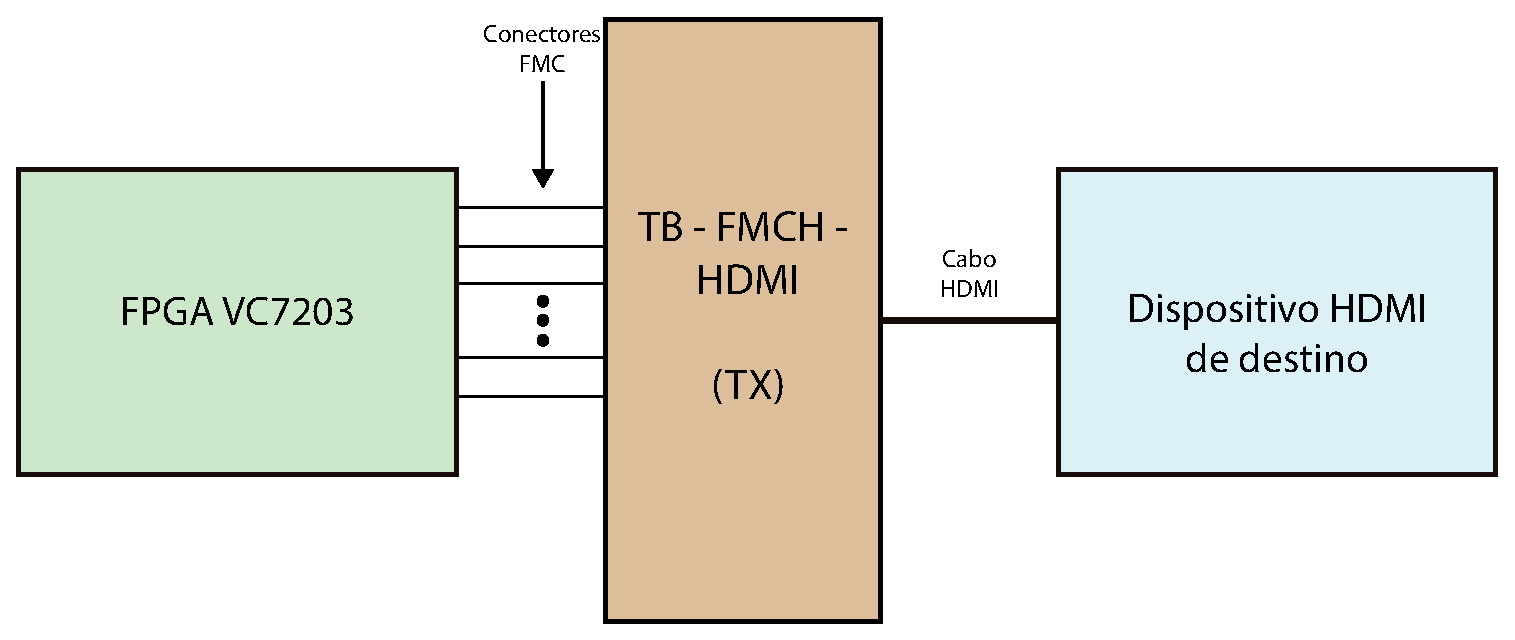
\includegraphics[width=0.8\textwidth]{planAsch}
		\caption{\textit{Setup} de teste da arquitetura desenvolvida para transmissão de uma imagem gerada na FPGA para a placa HDMI transmissora}
		\label{fig:planA_sch}
	\end{center}
\end{figure}

A figura \ref{fig:resultados_planoA} demonstra os resultados obtidos com a implementação desta arquitetura. A placa HDMI transmissora está conectada à FPGA através dos conectores FMC e ao dispositivo final através de um cabo HDMI. Com isto foi possível visualizar-se uma barra de cores no monitor, tal como esperado.

\begin{figure}[h!]
	\begin{center}
		\leavevmode
		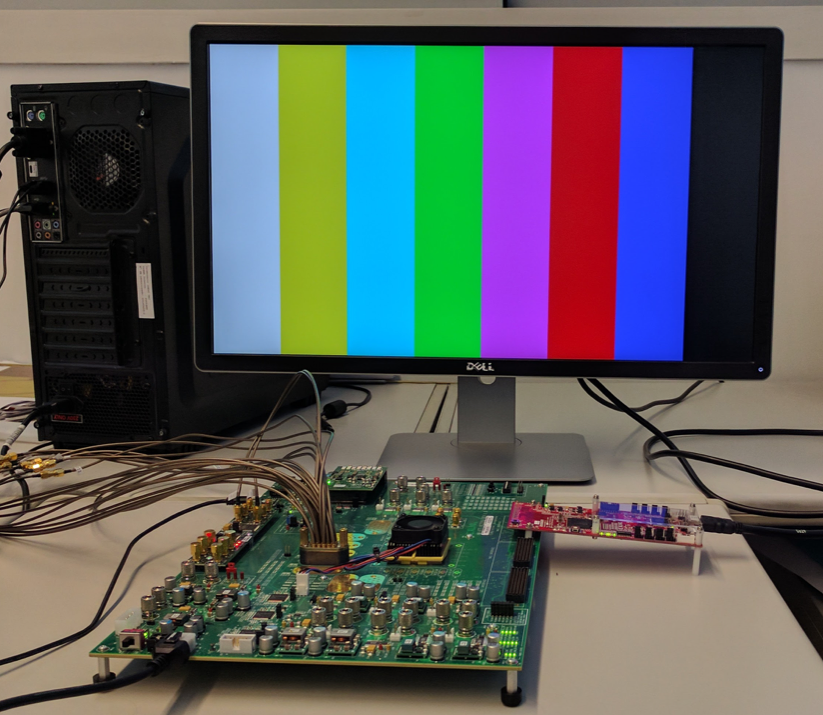
\includegraphics[width=0.6\textwidth]{resultados_planoA}
		\caption[Resultados obtidos da transmissão da barra de cores gerada na FPGA para o dispositivo de destino]{Resultados obtidos da transmissão da barra de cores gerada na FPGA para o dispositivo de destino}
		\label{fig:resultados_planoA}
	\end{center}
\end{figure}


\begin{center}
	\lrboxbrace[\Vert][\Vert] {}{
\textbf{Através da arquitetura implementada, a comunicação entre a FPGA e a placa HDMI transmissora foi bem sucedida, validando-se também o módulo desenvolvido para geração da barra de cores. Conclui-se assim, um passo intermédio que visa alcançar o objetivo final proposto na primeira parte do projeto.}}
\end{center}



\subsection{Transmissão de imagem entre dispositivos HDMI} \label{subsub:planB}

Na arquitetura desenvolvida que é apresentada nesta subsecção são utilizadas as placas HDMI recetora e transmissora, ambas configuradas por omissão e procede-se à transmissão de uma imagem entre dispositivos HDMI. O objetivo do desenvolvimento desta arquitetura consiste em obter uma ligação entre dois dispositivos ligados às placas HDMI de uma imagem RGB de 10 bits.

\subsubsection*{Conceção e Desenvolvimento}

Foi desenvolvida uma arquitetura que recebe à cadência do sinal de relógio HDMI proveniente da placa (neste caso em específico como é uma imagem \textit{FULL HD} é uma frequência de \SI{148.5}{\mega\hertz}) e o resto dos sinais provenientes da mesma, mais especificamente o valor de \textit{pixel}, \textit{vsync}, \textit{hsync} e \textit{enable}. A figura \ref{fig:planb1} ilustra o diagrama de blocos da arquitetura desenvolvida.

\begin{figure}[h!]
	\begin{center}
		\leavevmode
		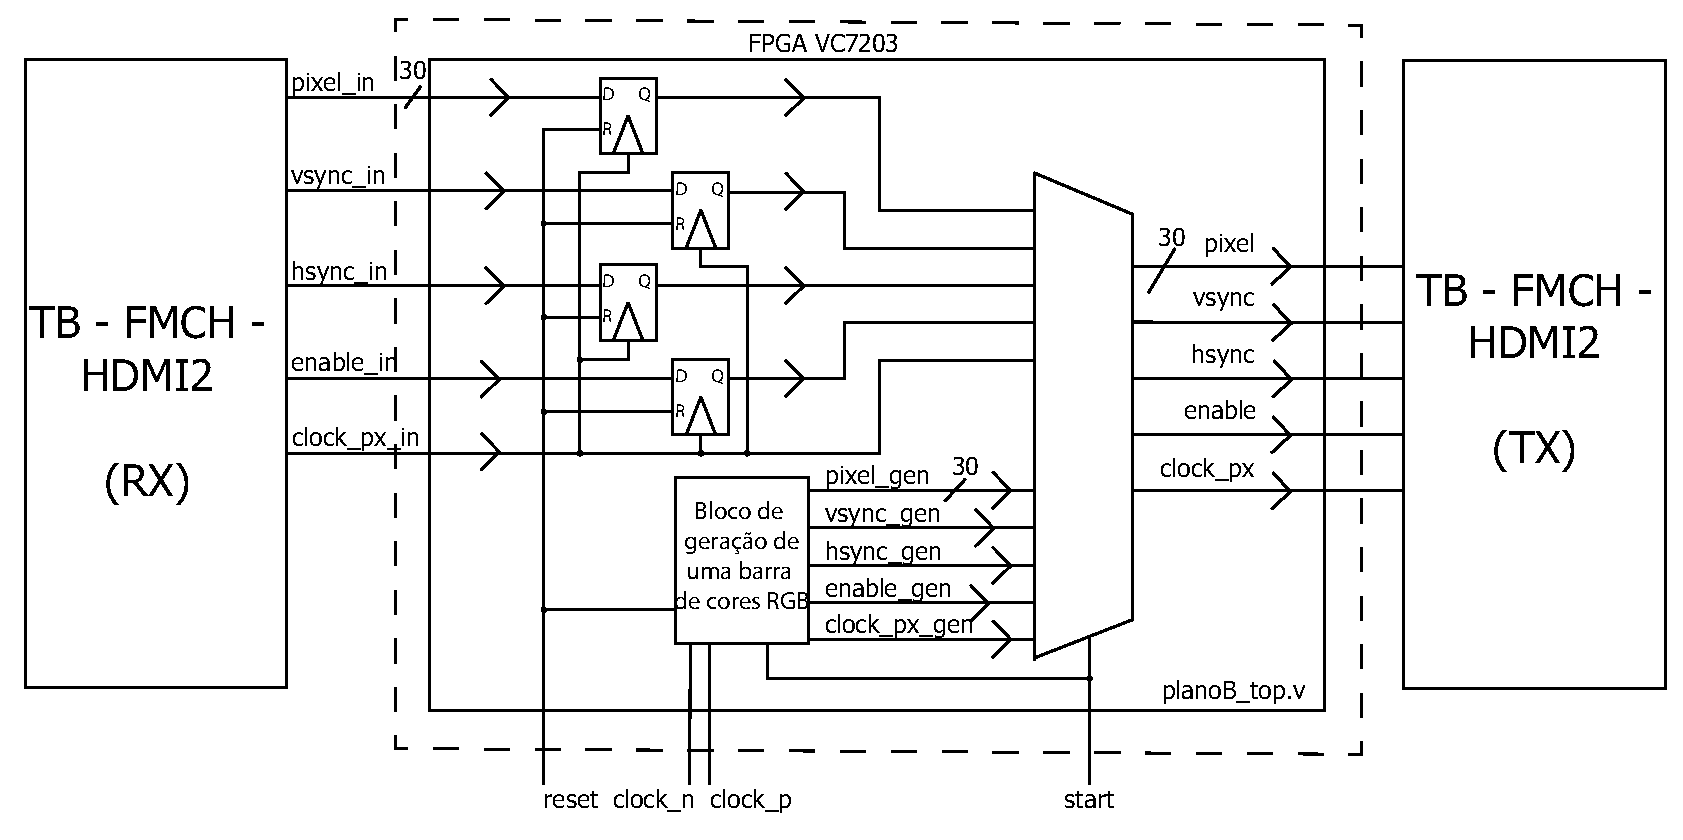
\includegraphics[width=1.0\textwidth]{planB1}
		\caption{Diagrama de blocos da arquitetura desenvolvida para transmitir imagem entre dispositivos HDMI}
		\label{fig:planb1}
	\end{center}
\end{figure}
%--> ENTRADA E SAIDA

É possível visualizar que na saída da arquitetura se encontram os sinais que são enviados para a placa HDMI transmissora. Por outro lado, além da presença dos sinais provenientes da placa HDMI recetora na entrada, existem ainda quatro outros sinais do exterior: o sinal de relógio diferencial de \SI{200}{\mega\hertz}, o sinal \textit{start} e \textit{reset}. O sinal de \textit{start} é definido pelo utilizador e seleciona os dados no multiplexador: quando ativo coloca na sua saída os dados provenientes do bloco gerador da barra de cores (anteriormente desenvolvido em \ref{subsub:planA}); quando inativo seleciona os dados recebidos da placa HDMI recetora. O sinal de \textit{reset} permite ao utilizador restabelecer os dados originais do sistema.

%--> FUNCIONAMENTO DA MESMA
Os sinais provenientes da placa HDMI recetora são lidos para registos síncronos com o flanco positivo do sinal de relógio da mesma. De seguida o multiplexador seleciona os sinais que são enviados para a placa HDMI transmissora consoante o valor de \textit{start}.

\subsubsection*{Localizações das portas de saída do módulo de topo} 

A tabela \ref{table:LOCplanB_simples} especifica as localizações físicas da FPGA que foram atribuídas a cada porta do módulo desenvolvido e ainda o banco ao qual pertencem. As portas que fazem conexão com as placas HDMI transmissora e recetora são apresentadas nesta tabela de forma abreviada. Contudo na secção \ref{ap3:imagem_RX_TX} do anexo \ref{ap3:LOCs} é possível encontrar mais detalhamente as localizações dessas portas na FPGA bem como informação relativamente a esses sinais nas placas HDMI transmissora e recetora.


\begin{table}[h!]
	\centering
		\caption{Localização das entradas e saídas das portas da arquitetura de transmissão de imagem entre dispositivos HDMI}
	\label{table:LOCplanB_simples}
%	\resizebox{\textwidth}{!}{%
		\begin{tabular}{rlll}
			\hline
			\multicolumn{1}{c}{\textbf{}}         & \multicolumn{1}{c}{\textbf{Sinal}}    & \multicolumn{1}{c}{\textbf{LOC na FPGA}} & \multicolumn{1}{c}{\textbf{Banco na FPGA}} \\ \hline
			\multicolumn{1}{r|}{\textbf{Entrada}} & clk\_p                                & E19                                      & 38                                         \\
			\multicolumn{1}{r|}{\textbf{Entrada}} & clk\_n                                & E18                                      & 38                                         \\
			\multicolumn{1}{r|}{\textbf{Entrada}} & reset                                 & N41                                      & 19                                         \\
			\multicolumn{1}{r|}{\textbf{Entrada}} & start                                 & E42                                      & 19                                         \\
			\multicolumn{1}{r|}{\textbf{Entrada}} & clk\_px\_in                           & AJ32                                     & 14                                         \\
			\multicolumn{1}{r|}{\textbf{Entrada}} & enable\_in                            & AN38                                     & 15                                         \\
			\multicolumn{1}{r|}{\textbf{Entrada}} & vsync\_in                             & AU38                                     & 15                                         \\
			\multicolumn{1}{r|}{\textbf{Entrada}} & hsync\_in                             & AU39                                     & 15                                         \\
			\multicolumn{1}{r|}{\textbf{Entrada}} & pixel\_in {[}0{]} a pixel\_in{[}29{]} & Ver anexo                                & 14 e 15                                    \\
			\multicolumn{1}{r|}{\textbf{Saída}}   & clk\_px                               & E34                                      & 35                                         \\
			\multicolumn{1}{r|}{\textbf{Saída}}   & enable                                & K35                                      & 34                                         \\
			\multicolumn{1}{r|}{\textbf{Saída}}   & hsync                                 & M32                                      & 34                                         \\
			\multicolumn{1}{r|}{\textbf{Saída}}   & vsync                                 & L31                                      & 34                                         \\
			\multicolumn{1}{r|}{\textbf{Saída}}   & pixel {[}0{]} a pixel {[}29{]}        & Ver anexo                                & 34 e 35                                    \\ \hline
		\end{tabular}%
\end{table}


%--> CONSTRAINTS %

A atribuição destas mesmas localizações das portas gerou um ficheiro de restrições físicas cujo conteúdo é apresentado nas secções \ref{ap:fisicas_deHDMI}, \ref{ap:fisicas_paraHDMI} e \ref{ap:fisicas_planB_especificas} do anexo \ref{ap2:codigo}. A secção \ref{ap:fisicas_deHDMI} define as portas de entrada que estão conectadas à placa HDMI recetora. A secção \ref{ap:fisicas_paraHDMI} apresenta as restrições das portas de saída da arquitetura que se conectam à placa HDMI transmissora, e por fim a secção \ref{ap:fisicas_planB_especificas} apresenta as restrições das restantes portas de entrada e saída desta arquitetura. As restrições temporais aplicadas à arquitetura são idênticas às que foram aplicadas anteriormente e estão presentes em \ref{ap:temporais_planB} no anexo \ref{ap2:codigo}.
%--> RESULTADOS

\subsubsection*{Resultados}
Após síntese e implementação do código desenvolvido em Verilog juntamente com as restrições aplicadas, a FPGA foi programada com esta arquitetura e testada recorrendo-se a um \textit{setup} de teste como ilustra a figura \ref{fig:planb_sch}. Foi utilizado um computador portátil como fonte HDMI e conectou-se o mesmo à placa recetora. Como dispositivo final utilizou-se um monitor que foi conectado à placa transmissora também com um cabo HDMI. 

\begin{figure}[h!]
	\begin{center}
		\leavevmode
		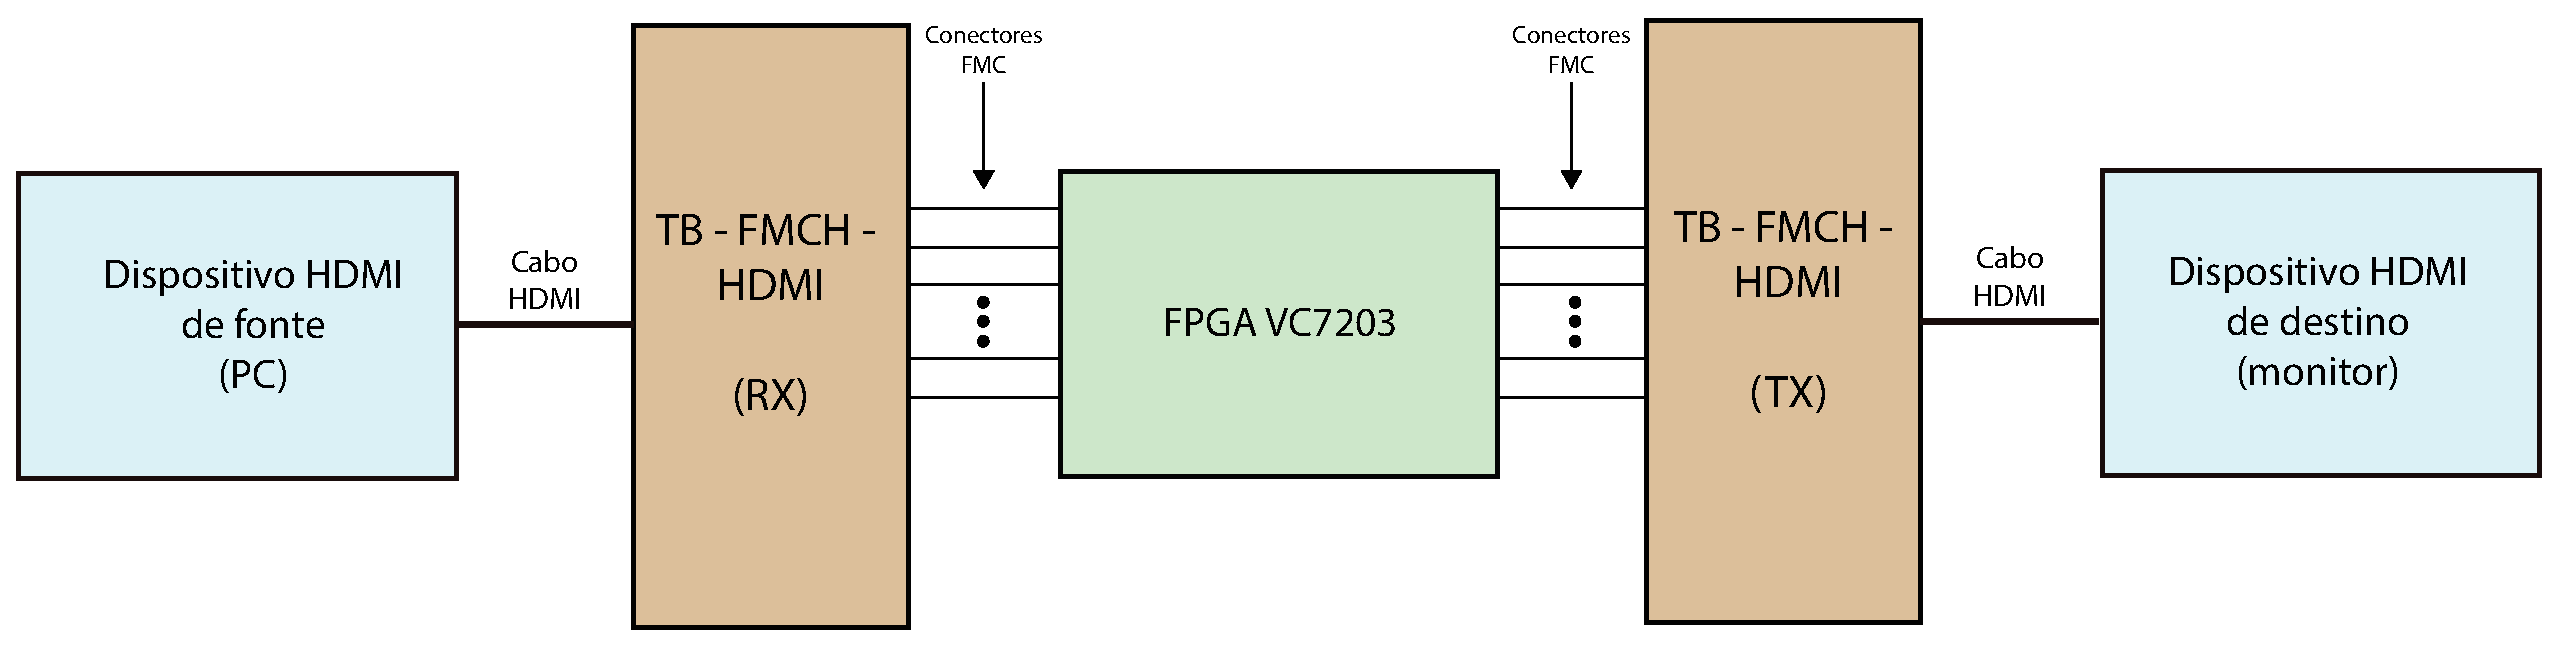
\includegraphics[width=1.0\textwidth]{planBsch}
		\caption{\textit{Setup} de teste para as arquiteturas transmissoras de dados entre dispositivos HDMI}
		\label{fig:planb_sch}
	\end{center}
\end{figure}

Na figura \ref{fig:resultados_planoB} visualizam-se os resultados obtidos com a implementação desta arquitetura: tal como esperado a imagem foi transmitida com sucesso.

\begin{figure}[h!]
	\begin{center}
		\leavevmode
		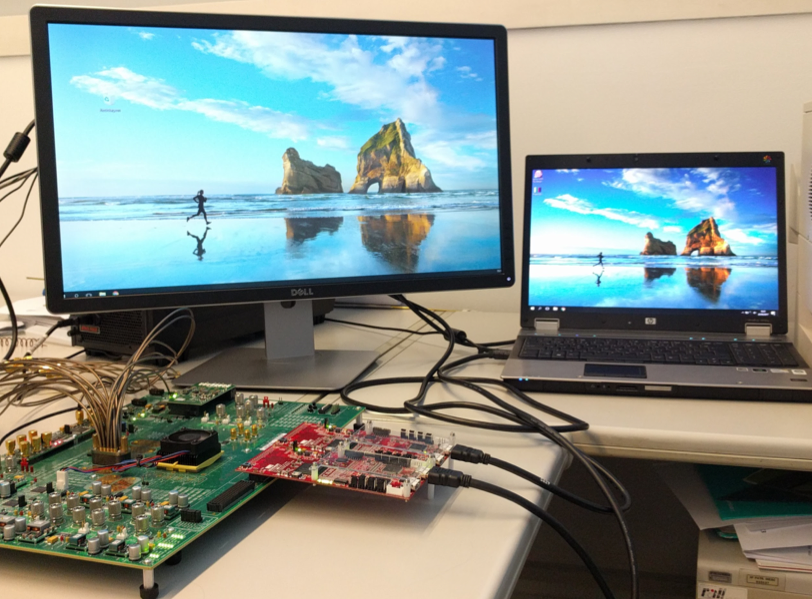
\includegraphics[width=0.5\textwidth]{resultados_planoB}
		\caption{Resultados obtidos da arquitetura transmissora de imagem entre dispositivos HDMI}
		\label{fig:resultados_planoB}
	\end{center}
\end{figure}

\begin{center}
\lrboxbrace[\Vert][\Vert] {}{
	\textbf{O último passo intermédio é assim concluído e permite alcançar o objetivo final proposto nesta primeira fase do projeto: a ligação entre dispositivos HDMI de fonte e destino foi obtida com sucesso.}}
\end{center}


\subsection{Transmissão de imagem e som entre dispositivos HDMI}

Após se obter uma ligação entre dois dispositivos HDMI de uma imagem procedeu-se ao desenvolvimento de uma arquitetura capaz de transmitir imagem e som. Para isso foi necessário reconfigurar as placas HDMI, tal como mencionado anteriormente, para a configuração que suporta apenas um canal mas que permite a transmissão de áudio em formato $I^{2}$S. As características desta configuração são apresentadas na subsecção \ref{subsubsec:HDMIconfig+audio} . É de notar que as imagens poderão ser transmitidas e recebidas em dois tipos de formatos (RGB ou YCbCr) e ainda com 8, 10 ou 12 bits por cor (dependendo da configuração dos interruptores das placas HDMI que estão especificados na secção \ref{sec:HDMIconfig+audio_switches} do anexo \ref{ap4:switches}). Neste caso específico são utilizados 12 bits por cor o que perfará um total de 36 bits por píxel.

\subsubsection*{Conceção e Desenvolvimento}

\begin{figure}[h!]
	\begin{center}
		\leavevmode
		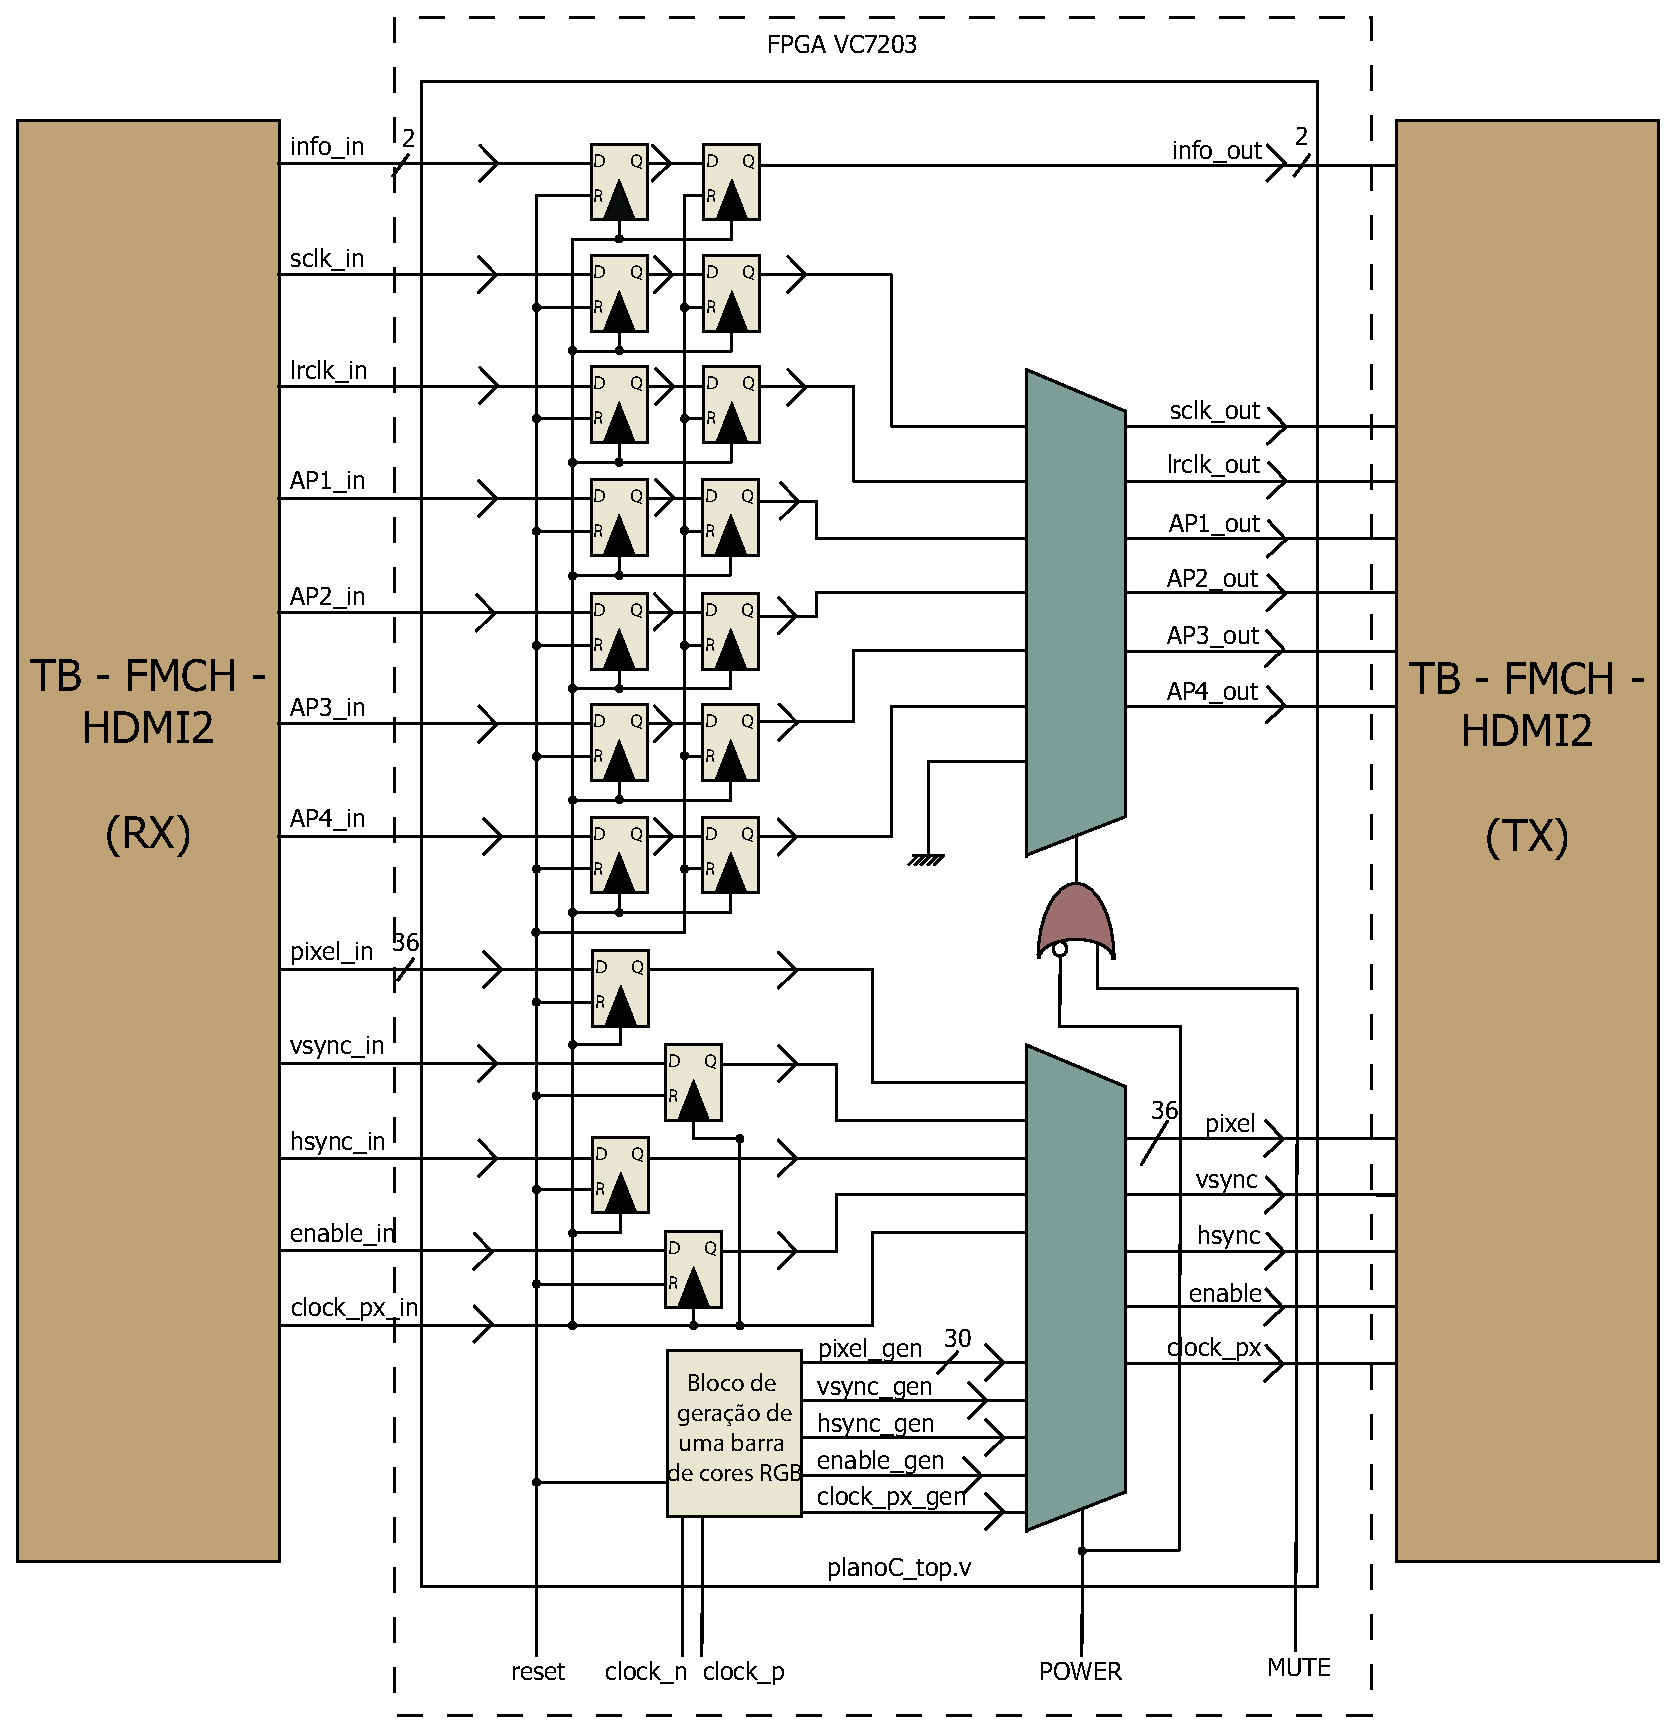
\includegraphics[width=1.0\textwidth]{planC}
		\caption{Diagrama de blocos da arquitetura desenvolvida para transmitir imagem e som entre dispositivos HDMI}
		\label{fig:planC}
	\end{center}
\end{figure}


Na figura \ref{fig:planC} é ilustrado o diagrama de blocos da arquitetura desenvolvida para se realizar a transmissão de imagem e som entre dois dispositivos HDMI. Facilmente se observa um número elevado de portas de entrada e saída nesta arquitetura, o que se deve ao facto de agora o som ser também transmitido.

%--> ENTRADA E SAIDA
Na entrada encontram-se os sinais relativos à imagem, à semelhança das arquiteturas anteriores: \textit{pixel}, \textit{hsync}, \textit{vsync}, \textit{enable} e o sinal de relógio da mesma. Para além destes sinais provenientes da placa HDMI recetora são ainda recebidos os sinais referentes ao som: o sinal de relógio dos dados em série (\textit{sclk}), o sinal referente à seleção do canal de áudio (\textit{lrclk}) e ainda os sinais que transportam os dados de som (de AP1 a AP4). Para além de dados de imagem e som há também um barramento de 2 bits que contém informação relativamente ao tipo de vídeo que é transmitido (tal como já referido na subsecção \ref{subsubsec:HDMIconfig+audio}). Todos estes sinais que se encontram na entrada do módulo, encontram-se também na saída pois são enviados para a placa HDMI transmissora.

Existem ainda outras três entradas do módulo : \textit{POWER}, \textit{MUTE} e \textit{reset}. O sinal de \textit{POWER} define o estado da transmissão (ativa ou desativa) e o sinal de \textit{MUTE} define a transmissão ou não dos sinais de som. O sinal de \textit{reset} serve para repor todos os dados originais do sistema caso o utilizador pretenda.
%% FUNCIONAMENTO DA MESMA

Os sinais de entrada relativos à imagem são lidos para registos síncronos com o flanco positivo do sinal de relógio de imagem. Estes mesmos sinais são enviados para a placa HDMI transmissora caso o sinal \textit{POWER} esteja ativo. Quando este sinal se encontra inativo suspende a transmissão.

Relativamente aos dados referentes ao som, estes são também lidos para registos síncronos com o flanco positivo do sinal de relógio referente à imagem proveniente da fonte HDMI. Numa fase mais avançada do projeto esta simplificação facilitará a transmissão dos dados em série a alta velocidade. Porém, é necessário ter em consideração que estes dados variam a uma taxa que não é síncrona com o sinal de relógio da imagem, pois este possui uma frequência de \SI{148.5}{\mega\hertz} para uma imagem no formato \textit{FULL HD} e os dados de som variam a uma frequência de \SI{3.072}{\mega\hertz} (tal como mencionado na subsecção \ref{subsubsec:HDMIconfig+audio}). Assim sendo, apesar de o sinal de relógio de áudio ser mais lento do que o da imagem, é necessário tomar as devidas precauções quando se faz a passagem entre estes dois domínios de relógio, para que não sejam captados dados dos registos quando estes se encontram num estado de meta-estabilidade. Tal como sugerido em \cite{R024}, são utilizados dois registos síncronos com o sinal de relógio referente à imagem para que não haja propagação de erros.

O sinal de áudio enviado para as placas HDMI transmissora está dependente dos sinais de \textit{POWER} e \textit{MUTE}. Caso \textit{MUTE} esteja ativo o sinal de som não é transmitido e as entradas da placa HDMI são definidas com 0. O mesmo acontece quando o sinal de \textit{POWER} está inativo uma vez que indica que a transmissão da parte da placa HDMI recetora está desligada.

\subsubsection*{Localizações das portas de saída do módulo de topo} 

Mais uma vez é necessário definir as localizações físicas de cada porta de entrada e saída do módulo principal, que estão descritas na tabela \ref{table:LOCplanC_simples}. Nessa mesma tabela os sinais que conectam as placas HDMI são brevemente apresentados e na secção \ref{ap3:imagem_som_RX_TX} do anexo \ref{ap3:LOCs} são descritos com mais detalhe.


\begin{table}[h!]
	\centering
	\caption{Localização das portas da arquitetura transmissora de imagem e som entre dispositivos HMDI}
	\label{table:LOCplanC_simples}
	\begin{tabular}{rlll}
		\hline
		\multicolumn{1}{c}{\textbf{}}         & \multicolumn{1}{c}{\textbf{Sinal}}    & \multicolumn{1}{c}{\textbf{LOC na FPGA}} & \multicolumn{1}{c}{\textbf{Banco na FPGA}} \\ \hline
		\multicolumn{1}{r|}{\textbf{Entrada}} & reset                                 & N41                                      & 19                                         \\
		\multicolumn{1}{r|}{\textbf{Entrada}} & POWER                                 & E42                                      & 19                                         \\
		\multicolumn{1}{r|}{\textbf{Entrada}} & MUTE                                  & G41                                      & 19                                         \\
		\multicolumn{1}{r|}{\textbf{Entrada}} & clk\_px\_in                           & AJ32                                     & 14                                         \\
		\multicolumn{1}{r|}{\textbf{Entrada}} & enable\_in                            & AN38                                     & 15                                         \\
		\multicolumn{1}{r|}{\textbf{Entrada}} & vsync\_in                             & AU38                                     & 15                                         \\
		\multicolumn{1}{r|}{\textbf{Entrada}} & hsync\_in                             & AU39                                     & 15                                         \\
		\multicolumn{1}{r|}{\textbf{Entrada}} & pixel\_in {[}0{]} a pixel\_in{[}29{]} & Ver anexo                                & 14 e 15                                    \\
		\multicolumn{1}{r|}{\textbf{Entrada}} & pixel\_in{[}30{]} a pixel\_in{[}35{]} & Ver anexo                                & 14                                         \\
		\multicolumn{1}{r|}{\textbf{Entrada}} & sclk\_in                              & AJ37                                     & 14                                         \\
		\multicolumn{1}{r|}{\textbf{Entrada}} & lrclk\_in                             & AL35                                     & 14                                         \\
		\multicolumn{1}{r|}{\textbf{Entrada}} & AP1\_in                               & AL37                                     & 14                                         \\
		\multicolumn{1}{r|}{\textbf{Entrada}} & AP2\_in                               & AP35                                     & 14                                         \\
		\multicolumn{1}{r|}{\textbf{Entrada}} & AP3\_in                               & AM37                                     & 14                                         \\
		\multicolumn{1}{r|}{\textbf{Entrada}} & AP4\_in                               & AH33                                     & 14                                         \\
		\multicolumn{1}{r|}{\textbf{Entrada}} & info\_in {[}0{]}                      & AV38                                     & 15                                         \\
		\multicolumn{1}{r|}{\textbf{Entrada}} & info\_in {[}1{]}                      & AV39                                     & 15                                         \\
		\multicolumn{1}{r|}{\textbf{Saída}}   & clk\_px                               & E34                                      & 35                                         \\
		\multicolumn{1}{r|}{\textbf{Saída}}   & enable                                & K35                                      & 34                                         \\
		\multicolumn{1}{r|}{\textbf{Saída}}   & hsync                                 & M32                                      & 34                                         \\
		\multicolumn{1}{r|}{\textbf{Saída}}   & vsync                                 & L31                                      & 34                                         \\
		\multicolumn{1}{r|}{\textbf{Saída}}   & pixel {[}0{]} a pixel {[}29{]}        & Ver anexo                                & 34 e 35                                    \\
		\multicolumn{1}{r|}{\textbf{Saída}}   & pixel {[}30{]} a pixel {[}35{]}       & Ver anexo                                & 35                                         \\
		\multicolumn{1}{r|}{\textbf{Saída}}   & sclk\_out                             & A34                                      & 35                                         \\
		\multicolumn{1}{r|}{\textbf{Saída}}   & lrclk\_out                            & B33                                      & 35                                         \\
		\multicolumn{1}{r|}{\textbf{Saída}}   & AP1\_out                              & A36                                      & 35                                         \\
		\multicolumn{1}{r|}{\textbf{Saída}}   & AP2\_out                              & C39                                      & 35                                         \\
		\multicolumn{1}{r|}{\textbf{Saída}}   & AP3\_out                              & B38                                      & 35                                         \\
		\multicolumn{1}{r|}{\textbf{Saída}}   & AP4\_out                              & D32                                      & 35                                         \\
		\multicolumn{1}{r|}{\textbf{Saída}}   & info\_out {[}0{]}                     & K32                                      & 34                                         \\
		\multicolumn{1}{r|}{\textbf{Saída}}   & info\_out {[}1{]}                     & L32                                      & 34                                         \\ \hline
	\end{tabular}
\end{table}

%--> CONSTRAINTS %

Para que a ferramenta de implementação reconheça as localizações físicas da FPGA atribuídas às portas do bloco é gerado um ficheiro de restrições físicas semelhante aos anteriores.

O conteúdo do ficheiro pode ser encontrado nas secções \ref{ap:fisicas_paraHDMI}, \ref{ap:fisicas_deHDMI} e ainda em \ref{ap:fisicas_planC_especificas} do anexo \ref{ap2:codigo}. Na secção \ref{ap:fisicas_paraHDMI} é possível encontrar as restrições físicas relativas a algumas portas de saída do módulo, nomeadamente os bits do sinal de píxel entre 0 e 29, o seu sinal de relógio e ainda os sinais de controlo de imagem. Na secção \ref{ap:fisicas_deHDMI} encontram-se as restrições físicas de algumas portas de entrada desta arquitetura provenientes da fonte HDMI. Essas portas correspondem, mais uma vez, aos bits do sinal de píxel entre 0 e 29, o seu sinal de relógio e os respetivos sinais de controlo. Por fim, em \ref{ap:fisicas_planC_especificas} encontram-se as restrições físicas referentes às restantes portas.


\subsubsection*{Resultados}

%--> RESULTADOS
%%POR IMAGEM DO SET_UP


Esta arquitetura foi devidamente implementada na FPGA e testada utilizando-se um \textit{setup} de teste semelhante ao que se visualiza na figura \ref{fig:planb_sch}, tendo em conta que o monitor utilizado neste teste tinha saída de áudio. 


Os resultados obtidos foram os esperados: a comunicação de imagem e som entre dois dispositivos foi conseguida. Os sinais de imagem e som operam à mesma frequência, tal como pretendido, para que possa facilitar a implementação da serialização destes dados. Apesar de os sinais de áudio provenientes da placa HDMI recetora serem síncronos com sinal de relógio que não é o dos píxeis, a passagem de sinais entre estes dois domínios de relógio não apresentou qualquer tipo de problema uma vez que ao ouvido humano os pequenos atrasados que possam eventualmente acontecer não são percetíveis .


\begin{center}
	\lrboxbrace[\Vert][\Vert] {}{
		\textbf{Com o objetivo final desta primeira fase já concluído, foi possível adicionar uma nova característica à mesma: o suporte de som. }}
\end{center}


\subsection{Análise dos recursos utilizados por cada uma das arquiteturas}

Nesta subsecção é apresentada uma análise dos recursos utilizados para cada uma das arquiteturas implementadas e retiradas algumas conclusões sobre as mesmas. 
Por questões de simplificação definiu-se:
\begin{itemize}
	\item \textbf{Arquitetura A:} Arquitetura transmissora de uma barra de cores para o dispositivo final HDMI;
	\item \textbf{Arquitetura B:} Arquitetura transmissora de imagem entre dispositivos HDMI;
	\item \textbf{Arquitetura C:} Arquitetura transmissora de imagem e som entre dispositivos HDMI.
\end{itemize}

\begin{table}[h!]
	\centering
	\caption{Recursos utilizados pelas diferentes arquiteturas implementadas na FPGA}
	\label{table:recursos_a_b_c}
	\resizebox{\textwidth}{!}} & \multicolumn{1}{c}{\textbf{Utilização}} & \multicolumn{1}{c|}{\textbf{\%}} & \multicolumn{1}{c}{\textbf{Utilização}} & \multicolumn{1}{c}{\textbf{\%}} \\ \hline
			\textbf{FF}                                            & 31                                      & 0,01                             & 64                                      & 0,01                            & 59                                      & 0,01                            \\
			\textbf{LUT}                                           & 59                                      & 0,02                             & 67                                      & 0,02                            & 27                                      & 0,01                            \\
			\textbf{I/O}                                           & 38                                      & 5,43                             & 70                                      & 10                               & 103                                     & 14,71                           \\
			\textbf{GT}                                            & 0                                       & 0                                & 0                                       & 0                                & 0                                       & 0                               \\ \hline
		\end{tabular}%
	}
\end{table}

Na tabela \ref{table:recursos_a_b_c} são apresentados a quantidade dos principais recursos utilizados em cada arquitetura desenvolvida. Estes dados foram retirados diretamente do \textit{software} após a implementação de cada arquitetura. 

Relativamente aos FF (\textit{Flip-Flop}) utilizados por cada uma das arquiteturas, através da análise destes dados, conclui-se que todas apresentam um número relativamente baixo. Tal como é de esperar, existe um aumento do mesmo da arquitetura A para a B que se relaciona com o facto de a arquitetura B receber dados provenientes da placa HDMI recetora e utilizar FF para os guardar. Este número baixa da arquitetura B para a C porque esta última não possui o bloco gerador da barra de cores. No geral, a utilização deste recurso não é preocupante nesta FPGA porque ainda existem muitos disponíveis.

O número de LUT (\textit{LookUp Tables}) usadas relacionam-se com a lógica combinacional utilizada na arquitetura. Como esperado, os valores resultantes da utilização deste recurso para todas as arquiteturas são relativamente baixos. Mais uma vez, para esta FPGA estes valores são muito baixos e ainda existem muitos que podem ser utilizados, não sendo relevante.

No que toca ao número de I/O (\textit{Inputs/Outputs}) utilizados em cada arquitetura, é possível observar uma crescente utilização de arquitetura para arquitetura, tal como é de esperar. Tal prende-se com o facto de o número de entradas e saídas das mesmas ir aumentando. Contudo, mesmo no caso C em que são usados $14,71\%$ dos recursos disponíveis, este valor não apresenta qualquer tipo de problema dada a FPGA em utilização.

De um ponto de vista geral a percentagem de recursos utilizados foi baixo, deixando a possibilidade de expandir o projeto caso se pretenda.


%FF -> 
%LUT -> logica combinacional utilizada
%I/O -> entradas e saidas
%BUFG -> buffer globais (provide the least amount of skew possible between registers that are physically located large distances apart)
%GT -> transcetores